We can think of a \emph{regionalism} as a word whose usage is not uniform across all the studied territory -- i.e., whose concentration is high in a specific region of the country. We are trying, in fact, to measure the \textit{disorder} in the usage of a word, and there exists a specific information-theoretic tool for this: entropy.

It is known that entropy holds information about the semantic role played by a word. Given a text, high-entropy words are more likely to be pronouns, connectors and other closed-class words, whereas its low-entropy counterparts are usually nouns and adjectives with fuller semantic content \cite{montemurro2002entropic, montemurro2010towards}. 

Taking into account their number of occurrences, words with high entropy (i.e,, high disorder) can be regarded as used evenly all across the country. On the other hand, low-entropy words are used with higher frequency in a few specific regions.

For a given word $\omega$, we define $p_k^\omega$ as the relative frequency of mentions of $\omega$ in a region $k$. It holds that $0 \leq p_k^\omega \leq 1$ and $\sum_{k=1}^N p_k^\omega = 1$, where $N$ is the number of regions (in our case, Argentina has $N=23$ provinces).
In other words, $p_k^\omega$ models the distribution of mentions of $\omega$ over all regions in the country. For example, if a given word was mentioned primarily in one particular region, then its value of $p_k^\omega$ will be close to 1 for that region and close to 0 for all other regions. 
We next define the \emph{word-count entropy} as
\begin{equation}
    H_\text{words}(\omega) = -\sum \limits_{k=1}^{N} p_k^{\omega} \cdot \log p_k^\omega
    \label{eqn:Hw}
\end{equation}

Note that this measure does not take into account the actual frequency of words. For instance, if two words $\omega_1$ and $\omega_2$ occur only in one particular region, but $\omega_1$ is much more frequent than $\omega_2$, both words will still have the same entropy according to Equation \ref{eqn:Hw}.
To remediate this issue, we developed a new measure that does take into account the frequency of words, inspired in \citet{montemurro2010towards}. We define the \wordmetric{} of $\omega$ as
\begin{equation}
  \label{eqn:iv_words}
  I_\text{words}(\omega) = p(\omega) \cdot (\log N  - H_\text{words}(\omega)),
\end{equation}
where $\log N$ is the maximum possible value of $H_\text{words}(\omega)$ \cite{shannon2001mathematical}, and $p(\omega)$ is the relative frequency of $\omega$ in the corpus ($0 \leq p(\omega) \leq 1$). In this way, $I_\text{words}(\omega)$ will be high for frequent words that accumulate in just a few regions.

Another important aspect of a word is the amount of people using it on Twitter, something already used in  \citet{Cui:2012:DBE:2396761.2398519}. For a given word $\omega$, we now define $q_k^\omega$ as the proportion of users who mentioned $\omega$ that live in region $k$. Again, it holds that $0 \leq q_k^\omega \leq 1$ and $\sum_{k=1}^N q_k^\omega = 1$.
In this case, $q_k^\omega$ models the distribution of users who mentioned $\omega$ over all regions in the country. For example, if a given word was mentioned primarily by users from one particular region, then its value of $q_k^\omega$ will be close to 1 for that region and close to 0 for all other regions.  We define the \emph{user-count entropy} as
\begin{equation}
    H_\text{users}(\omega) = -\sum \limits_{k=1}^{N} q_k^{\omega} \cdot \log q_k^{\omega}
\end{equation}
and the \usermetric{} of  $\omega$ as
\begin{equation}
  \label{eqn:iv_users}
  I_\text{users}(\omega) = q(\omega) \cdot (\log N - H_\text{users}(\omega)),
\end{equation}
where $q(\omega)$ is the proportion of users who mentioned $\omega$ in the corpus ($0 \leq q(\omega) \leq 1$). Note that $I_\text{users}(\omega)$ will be high for words mentioned by several users who accumulate in just a few regions.

Figure \ref{fig:entropies} shows the distributions of \wordentropy{} and \userentropy{} for all words in our corpus. As one would expect, most words have a high entropy -- i.e. were used uniformly across the country, both in occurrences and in users.

According to Zipf's Law, the frequencies of top-used words are many orders of magnitude higher than others -- a phenomenon also true when counting users of words. So the $p(\omega)$ and $q(\omega)$ terms in equations \eqref{eqn:iv_words} and \eqref{eqn:iv_users} become a problem as words with high frequencies overcome their low entropies. To alleviate this, we performed a normalization on the word frequency as follows. Let $M_\omega$ be the most-frequent word, that is,
\begin{equation}
    M_\omega = \argmax\limits_{\omega \in W} \#\omega,
\end{equation}
where $\#\omega$ denotes the total number of occurrences of $\omega$ in our dataset. Then, the \emph{Normalized log-frequency} of word occurrences is defined as
\begin{equation}
    n_\text{words}(\omega) = \frac{\log(\# \omega)}{\log(\# M_w)}
\end{equation}

Words with very high frequency differ little on their values of $n_\text{words}(\omega)$. We define analogously the \emph{Normalized log-frequency} of user mentions $n_{users}$. Hence, we redefine our two metrics as
\begin{align}
  I_\text{words}(\omega) &= n_\text{words}(\omega) (\log(n) - H_\text{words}(\omega)) \\
  I_\text{users}(\omega) &= n_\text{users}(\omega) (\log(n) - H_\text{users}(\omega)) 
\end{align}

Finally, we combine our \emph{word-counts} and \emph{user-counts} metrics into a \mixedmetric{}, defined as
\begin{equation}
  I(\omega) = I_\text{words}(\omega) \cdot I_\text{users}(\omega)
\end{equation}
Now, $I(\omega)$ will be high for frequent words whose usage (in terms of both occurrences and users) accumulates in just a few regions.

A word having a high value for the metrics just defined may be regarded as being more present in a certain region than in the rest of the country. We subsequently sort all words in our dataset relative to these metrics, thus obtaining three word rankings: \wordrank{}, \userrank{} and
\mixedrank{}. The words that appear in the first positions of a ranking are those with high values for the metric, and thus more likely to be regionalisms.




\begin{figure}[h]
\centering
\begin{subfigure}[t]{0.45\textwidth}
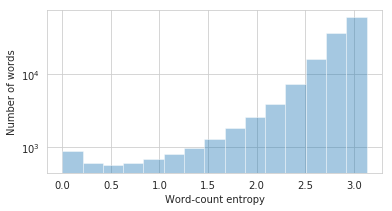
\includegraphics[width=\textwidth]{./images/word_count_entropy.png}
\caption{\label{fig:word_count_entropy}}
\end{subfigure}
\begin{subfigure}[t]{0.45\textwidth}
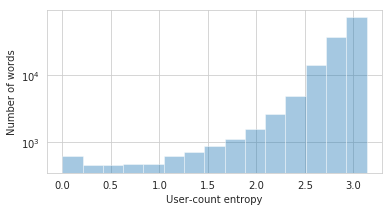
\includegraphics[width=\textwidth]{./images/user_count_entropy.png}
\caption{\label{fig:user_count_entropy}}
\end{subfigure}

\caption{Entropy histograms for words in our corpus. (\subref{fig:word_count_entropy}) Word-count entropy $H_\text{words}$ (entropy of words with respect to their usage per region).
(\subref{fig:user_count_entropy})
User-count entropy $H_\text{users}$ (entropy of words with respect to the regions of users who mentioned it).} 

\label{fig:entropies}

\end{figure}

\subsection{Lexicographic Validation}

With these rankings, a team of lexicographers from XXXX performed a linguistic validation of the first thousand words according to each metric. This qualitative analysis consisted in a detailed study, word by word, to determine if the word in question is part of the lexical repertoire of a community of speakers. Proper and place names (toponyms) were excluded --as is traditional in lexicography-- although many words in this class had high values for our metrics. 
%%AG: decir cómo se hizo esto de "suspected toponyms"
To facilitate the exclusion of regionalisms by lexicographers, words suspected of being toponyms were automatically highlighted.

To perform the linguistic validation, lexicographers were provided with tables containing figures for each word and province: number of users, number of occurrences and normalized frequency (occurrences per million words). Also, samples of tweets containing these words were provided when necessary. 

As a result of this process, every word in the top-1000 of each ranking was annotated with `1' if it had lexical relevance as a regionalism, or `0' if it had not. Lastly, lexicographers performed a characterization of the words marked as regionalisms, according to the linguistic phenomenon they represent. The outcome of these procedures is described in the following sections.
